\documentclass[a4paper, 10pt, final, garamond]{book}
\usepackage{cours-preambule}
\graphicspath{{./figures/}}
\addto\captionsfrench{\renewcommand{\figurename}{Fig.}}

\makeatletter
\renewcommand{\@chapapp}{Contr\^ole de connaissances}
\makeatother

% \toggletrue{student}
% \toggletrue{corrige}
\renewcommand{\mycol}{black}
% \renewcommand{\mycol}{gray}

\hfuzz=5.002pt

\begin{document}
\setcounter{chapter}{3}

\settype{enon}
\settype{solu}

\chapter{Électrocinétique~: premier ordre\ifstudent{~(15')}}

\begin{enumerate}[label=\sqenumi, leftmargin=10pt]
	\item[n]{2.5} %
	      Représenter et flécher $R_1$ et $R_2$ en parallèle et le schéma équivalent
	      avec $R\ind{eq}$. Démontrer son expression.
	      \smallbreak
	      \begin{isd}[lefthand ratio=.3]
		      \vspace{-15pt}
		      \begin{center}
			      \sswitch{%
				      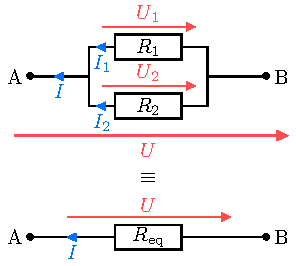
\includegraphics[width=.7\linewidth, draft=true]{rpara}
			      }{%
				      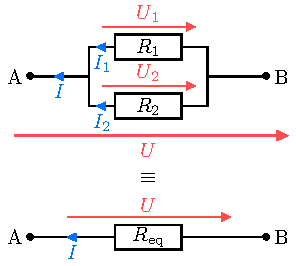
\includegraphics[width=.7\linewidth]{rpara}
			      }%
			      % \vspace{-15pt}
			      \captionof{figure}{$R$ parallèle \protect\pt{.5}\psw{+}\protect\pt{.5}}
		      \end{center}
		      \vspace{-15pt}
		      \tcblower
		      \vspace{-15pt}
		      \psw{%
			      \begin{align*}
				      I                   & \stm".5"{=}
				      I_1 + I_2 =
				      \left( \frac{1}{R_1} + \frac{1}{R_2} \right)U
				      \\\Lra
				      \frac{1}{R\ind{eq}} & \stm".5"{=}
				      \left( \frac{1}{R_1} + \frac{1}{R_2} \right)
				      \\\Lra
				      \Aboxed{R_{\rm eq}  & \stm".5"{=} \frac{R_1R_2}{R_1+R_2}}
				      \qed
			      \end{align*}
		      }%
		      \vspace{-15pt}
	      \end{isd}
	\item[n]{2.5} %
	      Représenter un pont diviseur de tension avec 2 résistances et démontrer la
	      relation associée pour des résistances $R_k$.
	      \smallbreak
	      \begin{isd}[lefthand ratio=.30]
		      \vspace{-15pt}
		      \begin{center}
			      \sswitch{%
				      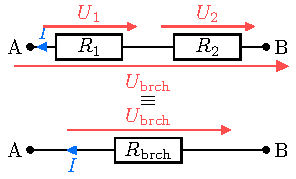
\includegraphics[width=\linewidth, draft=true]{rserie_divtens}
			      }{%
				      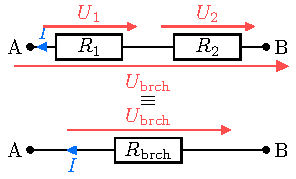
\includegraphics[width=\linewidth]{rserie_divtens}
			      }%
			      \vspace{-15pt}
			      \captionof{figure}{PdT \protect\pt{.5}\psw{+}\protect\pt{.5}}
		      \end{center}
		      \tcblower
		      \psw{%
			      On part de ce qui est partagé dans le circuit, ici l'intensité~:
			      \begin{gather*}
				      I = \frac{U\ind{brch}}{R\ind{brch}}
				      \stm".5"{\stm(un)".5"{\qet}}
				      I = \frac{U_k}{R_k}
				      \qqso
				      \boxed{U_k \stm".5"{=} \frac{R_k}{R\ind{brch}}U\ind{brch}}
				      \qed
			      \end{gather*}
		      }%
		      \vspace{-15pt}
	      \end{isd}
	\item[n]{15} %
	      \noindent
	      \begin{minipage}[t]{.69\linewidth}
		      On suppose le circuit RC série suivant, en échelon de tension montant. On
		      suppose le condensateur initialement déchargé, et on ferme l'interupteur à
		      $t=0$. Déterminer l'équation différentielle sous forme canonique de $u_C$
		      pour $t \geq 0$, donner la condition initiale et comment la déterminer, et
		      résoudre l'équation différentielle.
	      \end{minipage}
	      \hfill
	      \begin{minipage}[t]{.29\linewidth}
		      ~
		      \vspace{-30pt}
		      \begin{center}
			      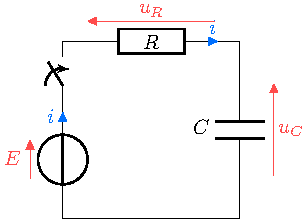
\includegraphics[width=.7\linewidth]{circ_rc-start}
			      \captionof{figure}{}
		      \end{center}
	      \end{minipage}
	      \begin{isd}[sidebyside align=top]
		      \psw{%
		      Avec la loi des mailles,
		      \begin{DispWithArrows*}
			      u_R + u_C &\stm{=} E
			      \Arrow{$u_R = Ri$\\et $i \stm(un){=} C \dv{u_C}{t}$}
			      \\\Lra
			      RC \dv{u_C}{t} + u_C        & = E
			      \Arrow{$\tau \stm{=} RC$}
			      \\\Lra
			      \dv{u_C}{t} + \frac{1}{\tau}u_C & \stm{=} \frac{E}{\tau}
		      \end{DispWithArrows*}
		      L'équation homogène est~:
		      \[
			      \dv{u_{C,h}}{t} + \frac{1}{\tau}u_{C,h} \stm{=} 0
		      \]
		      On injecte la forme générique de solutions, $u_{C,h}(t) \stm[-1]{=} K
			      \exr^{rt}$~:
		      \[
			      r \times \cancel{K \exr^{rt}} + \frac{\cancel{K \exr^{rt}}}{\tau} = 0
			      \Lra
			      r \stm{=} -\frac{1}{\tau}
		      \]
		      La forme générale de la solution pour cette équation est donc~:
		      \[
			      u_{C,h}(t) \stm{=} K\exp\left( -\frac{t}{\tau} \right)
		      \]
		      }%
		      \tcblower
		      \psw{%
			      Une solution particulière avec $u_{C,p}(t) = \lambda$ donne
			      \[
				      0 + \frac{\lambda}{\tau} \stm{=} \frac{E}{\tau}
			      \]
			      Donc $u_{C,p}(t) = E$ est \textbf{une} solution de l'équation
			      différentielle.
			      La solution générale est donc
			      \[
				      u_C(t) \stm{=} u_{C,h}(t) + u_{C,p}(t) \stm{=}
				      E + A\exp \left( - \frac{t}{\tau} \right)
			      \]
			      La condition initiale est, par continuité de $u_C(t)$ \pt{1},
			      \[
				      u_C(0^+) = u_C(0^-) \stm{=} 0 = A+E
				      \Lra
				      A \stm{=} -E
			      \]
			      Ainsi,
			      \[
				      \boxed{u_C(t) \stm{=} E\left(1-\exp\left(-\frac{t}{\tau}\right)\right)}
			      \]
		      }%
	      \end{isd}
\end{enumerate}
% \vspace{-15pt}

\ifstudent{%
	\begin{tikzpicture}[remember picture, overlay]
		\node[anchor=north west, align=left]
		at ([shift={(1.4cm,0)}]current page.north west)
		{\\[5pt]\Large\bfseries Nom~:\\[10pt]\Large\bfseries Prénom~:};
		\node[anchor=north east, align=right]
		at ([shift={(-1.5cm,-17pt)}]current page.north east)
		{\Large\bfseries Note~:\hspace{1cm}/20};
	\end{tikzpicture}
}%
\end{document}
